%----------------------------------------------------------------------------------------
%	PACKAGES AND THEMES
%----------------------------------------------------------------------------------------
\documentclass[aspectratio=169,xcolor=dvipsnames]{beamer}
\usetheme{SimplePlus}

\usepackage{hyperref}
\usepackage{graphicx} % Allows including images
\usepackage{booktabs} % Allows the use of \toprule, \midrule and \bottomrule in tables
\usepackage{wrapfig}
\usepackage{multimedia}
\usepackage{bm}
\usepackage{amsmath}
\usepackage{nicematrix}
\NiceMatrixOptions{
code-for-first-row = \color{blue} ,
code-for-last-row = \color{blue} ,
code-for-first-col = \color{blue} ,
code-for-last-col = \color{blue}
}

%----------------------------------------------------------------------------------------
%	TITLE PAGE
%----------------------------------------------------------------------------------------

\title[Higher-order Cheeger Inequalities]{Higher-order Cheeger Inequalities} % The short title appears at the bottom of every slide, the full title is only on the title page
\subtitle{Spectral Graph Theory}

\author[Taylor]{Matt Taylor}

\institute[UoB] % Your institution as it will appear on the bottom of every slide, may be shorthand to save space
{
    University of Bristol
}
\date{March 31, 2022} % Date, can be changed to a custom date


%----------------------------------------------------------------------------------------
%	PRESENTATION SLIDES
%----------------------------------------------------------------------------------------

\begin{document}

\begin{frame}
    % Print the title page as the first slide
    \titlepage
\end{frame}

%------------------------------------------------
\section{Introduction and Motivation}

% todo: eigenvectors non-zero in slide 5
% todo: eigenvalues of components are union of ..

\begin{frame}[c]{Graphs}
\begin{columns}

\begin{column}{0.6\textwidth}
\begin{center}
\begin{itemize}
\Large
\item $G = (V, E)$
\pause \item e.g: $V = \{a, b, c, d\}$ \only<4>{ \hspace{1em} \small(Let $n = |V|$.) }
\Large
\item[] \hspace{1.7em} $E = \{ \{a, c\}, \{b, c\}, \{c, d\} \}$
\end{itemize}
\end{center}
\end{column}

\begin{column}{0.4\textwidth}
\centering
\hspace{-5em}
\pause 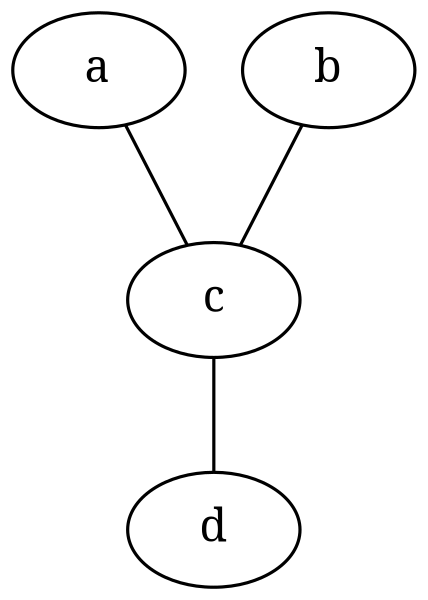
\includegraphics[width=0.7\textwidth]{graph-simple}
\end{column}

\end{columns}
\end{frame}

\begin{frame}{Laplacian Matrix}
% todo: mention that this is a discrete analogue of the continous operator for differential equations
% todo: DEFINITION NOT TOO IMPORTANT, just know that matrix captures information about the graph
\begin{columns}
% todo: we will now define some matrices associated with these graphs

\begin{column}{0.4\textwidth}
\centering
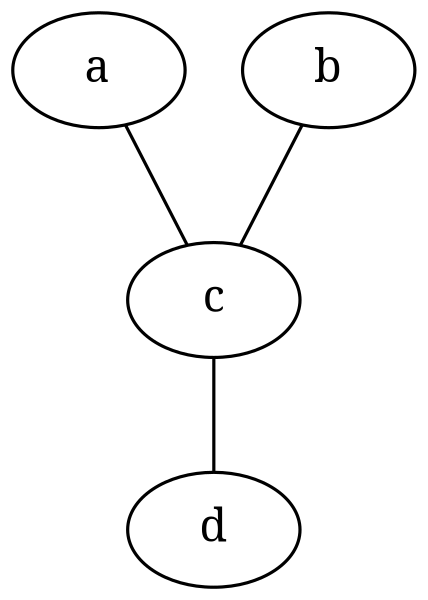
\includegraphics[width=0.7\textwidth]{graph-simple}
\end{column}

\begin{column}{0.6\textwidth}
\hspace{-1em}
\alt<4-5>{
\[
\hspace{-3em}
\alert{L} = D - A = \begin{pNiceMatrix}[first-row,first-col]
  & a & b & c & d \\
a & \phantom{-}1 & \phantom{-}0 & -1 & \phantom{-}0 \\
b & \phantom{-}0 & \phantom{-}1 & -1 & \phantom{-}0 \\
c & -1 & -1 & \phantom{-}3 & -1 \\
d & \phantom{-}0 & \phantom{-}0 & -1 & \phantom{-}1
\end{pNiceMatrix}
\]
\onslide<5>
\hspace{-4em}
\vspace{1em}
\[\text{Normalized: } \mathcal{\alert{L}} = D^{-1/2}LD^{-1/2}\]
}
{
\onslide<2-3>
\[
A = \begin{pNiceMatrix}[first-row,first-col]
  & a & b & c & d \\
a & 0 & 0 & 1 & 0 \\
b & 0 & 0 & 1 & 0 \\
c & 1 & 1 & 0 & 1 \\
d & 0 & 0 & 1 & 0
\end{pNiceMatrix}
\]
\onslide<3>
\[
D = \begin{pNiceMatrix}[first-col]
a & 1 & 0 & 0 & 0 \\
b & 0 & 1 & 0 & 0 \\
c & 0 & 0 & 3 & 0 \\
d & 0 & 0 & 0 & 1
\end{pNiceMatrix}
\]
}
\end{column}

\end{columns}

% todo: mention that this matrix is the main object of study in spectral graph theory.
\end{frame}

\begin{frame}{Spectrum of a Graph}
\centering
\Large
Interested in the Eigenvalues of $L$. \\\vspace{2em}
\large
\pause\text{Eigen\alert{values} of }L \hspace{1em} $0 = \lambda_1 \le \lambda_2 \le \dots \le \lambda_n$ \\
\pause\hspace{-0.20em}\text{Eigen\alert{vectors} of }L \hspace{2.9em} $f_1 \hspace{1.6em} f_2 \hspace{1.35em} \dots \hspace{1.25em} f_n$
\end{frame}


\begin{frame}{Eigenvalues of Laplacian}
%todo: mention: Interested in the eigenvalues of $L$.
% todo: mention that n x n matrix, where n = |V|
% todo: mention that lambda_1 = 0 ALWAYS (justify)?
\large
\begin{columns}
\begin{column}{0.6\textwidth}
\[
L = \begin{pNiceMatrix}[first-row,first-col]
  & a & b & c & d \\
a & \phantom{-}1 & \phantom{-}0 & -1 & \phantom{-}0 \\
b & \phantom{-}0 & \phantom{-}1 & -1 & \phantom{-}0 \\
c & -1 & -1 & \phantom{-}3 & -1 \\
d & \phantom{-}0 & \phantom{-}0 & -1 & \phantom{-}1
\end{pNiceMatrix}
\]
\vspace{1em}
\[\pause\lambda_2 = 0 \iff G \text{ is \alert{disconnected}.}\]
\end{column}

\begin{column}{0.4\textwidth}
\pause
\hspace{-4em}
\centering
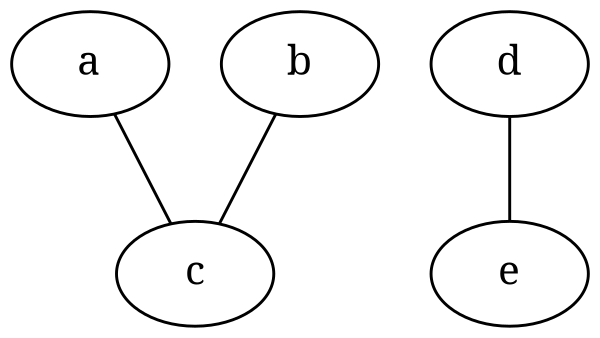
\includegraphics[width=0.8\textwidth]{graph-disconnected}
\end{column}

\end{columns}
\end{frame}

\begin{frame}{Eigenvectors as an Optimization Problem}
\vspace{-1em}
\centering
Relationship between $\lambda_2$ and arbitrary $f \in \mathbb{R}^n$ (i.e $f: V \to \mathbb{R}$). \\
\vspace{1em}\pause
\textbf{Courant-Fischer Theorem}:
\[
\lambda_2 = \alert{\min_{\bm{1} \perp f \in \mathbb{R}^n}}
\frac{\displaystyle\alert{\sum_{\{x, y\} \in E} (f(x) - f(y))^2}}{\displaystyle\sum_{v \in V} f(v)^2}
\]
$f_2$ is the vector which minimizes the above.
% todo: use image example to explain 
% todo: f_2 assigns value to each vertex... difference btw neighbours is minimized
% todo: mention 'does f_2(x) tell us anything interesting about x'
\end{frame}

\begin{frame}{Graph Drawing Problem}
\centering
For a general graph, how can we draw it? (map $V \to \mathbb{R}^2$)

\pause \alert{One way}: \textbf{Map each $v \in V$ to random point in $\mathbb{R}^2$}
% todo: mention drawing edges as straight lines!!!!
% todo: mention n = 50

\pause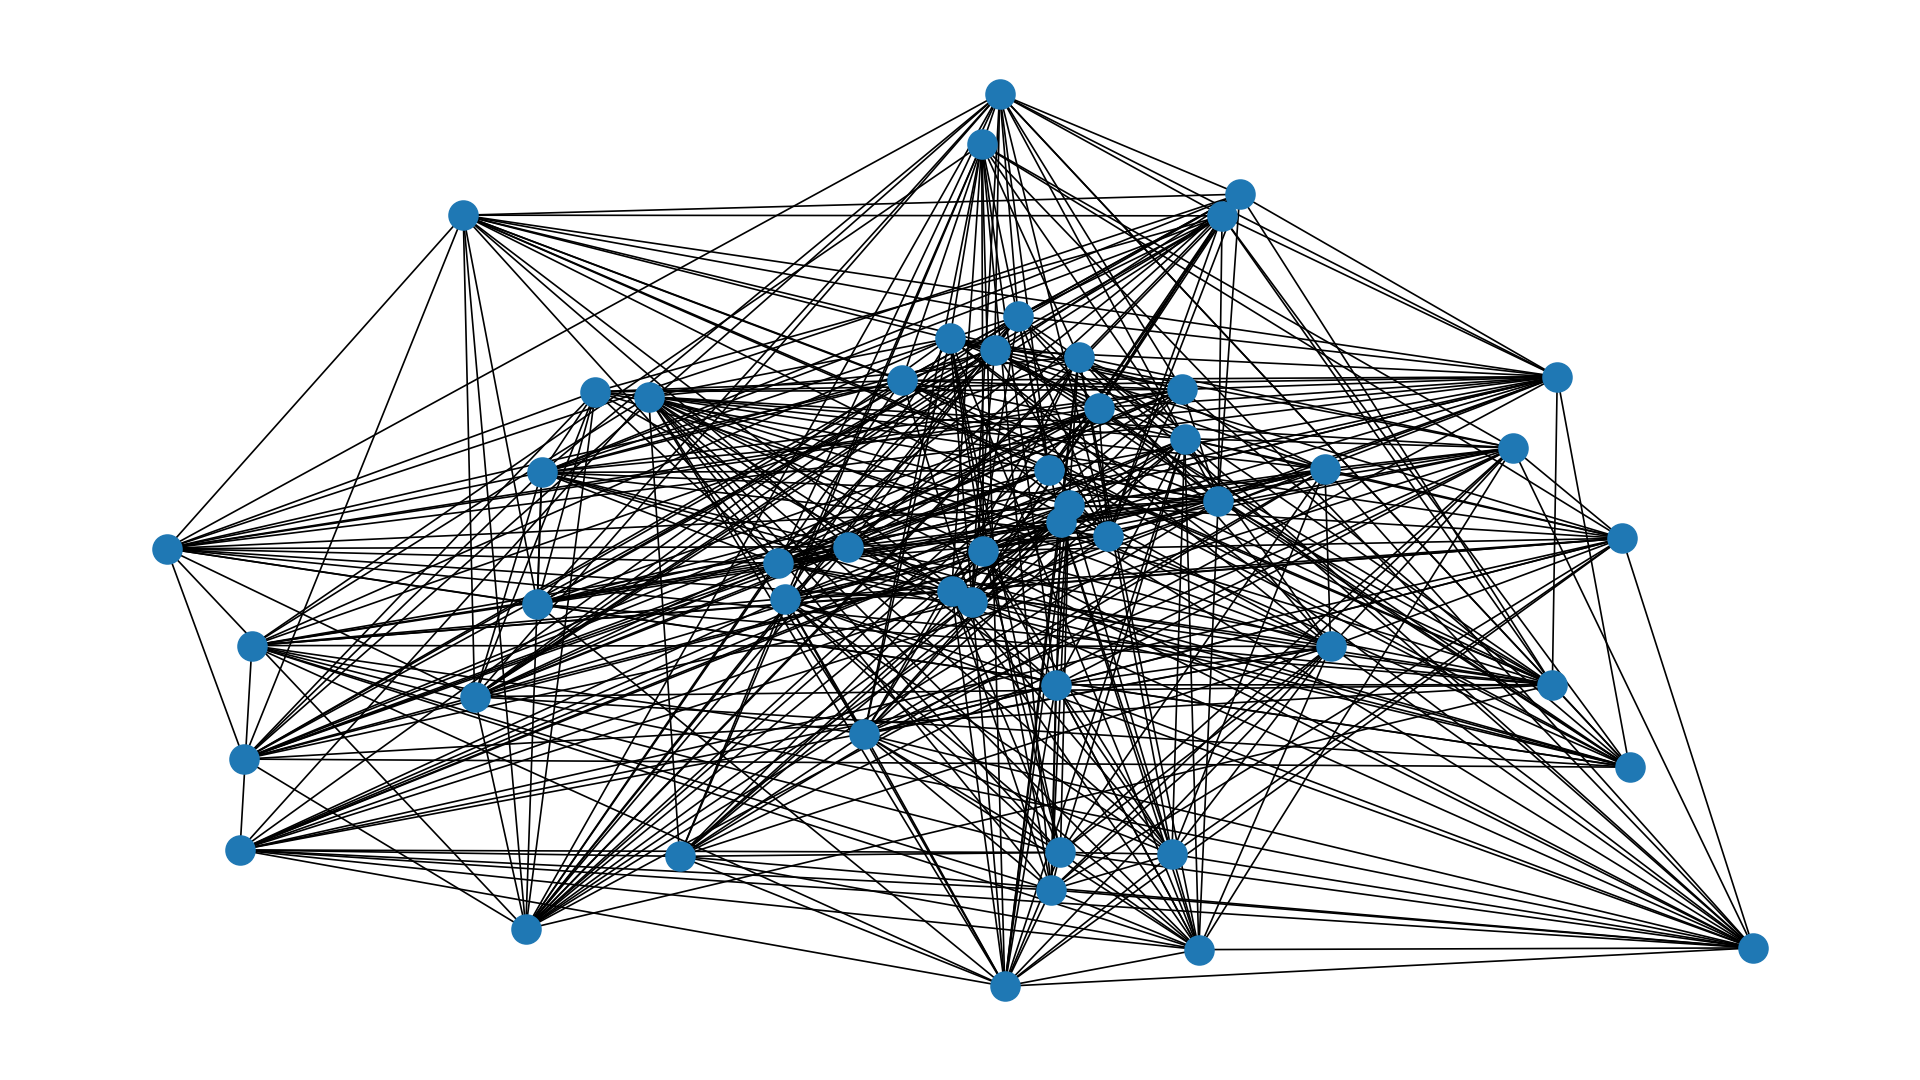
\includegraphics[width=0.75\textwidth]{anim-0}
\end{frame}

\begin{frame}{Graph Drawing Problem}
\centering
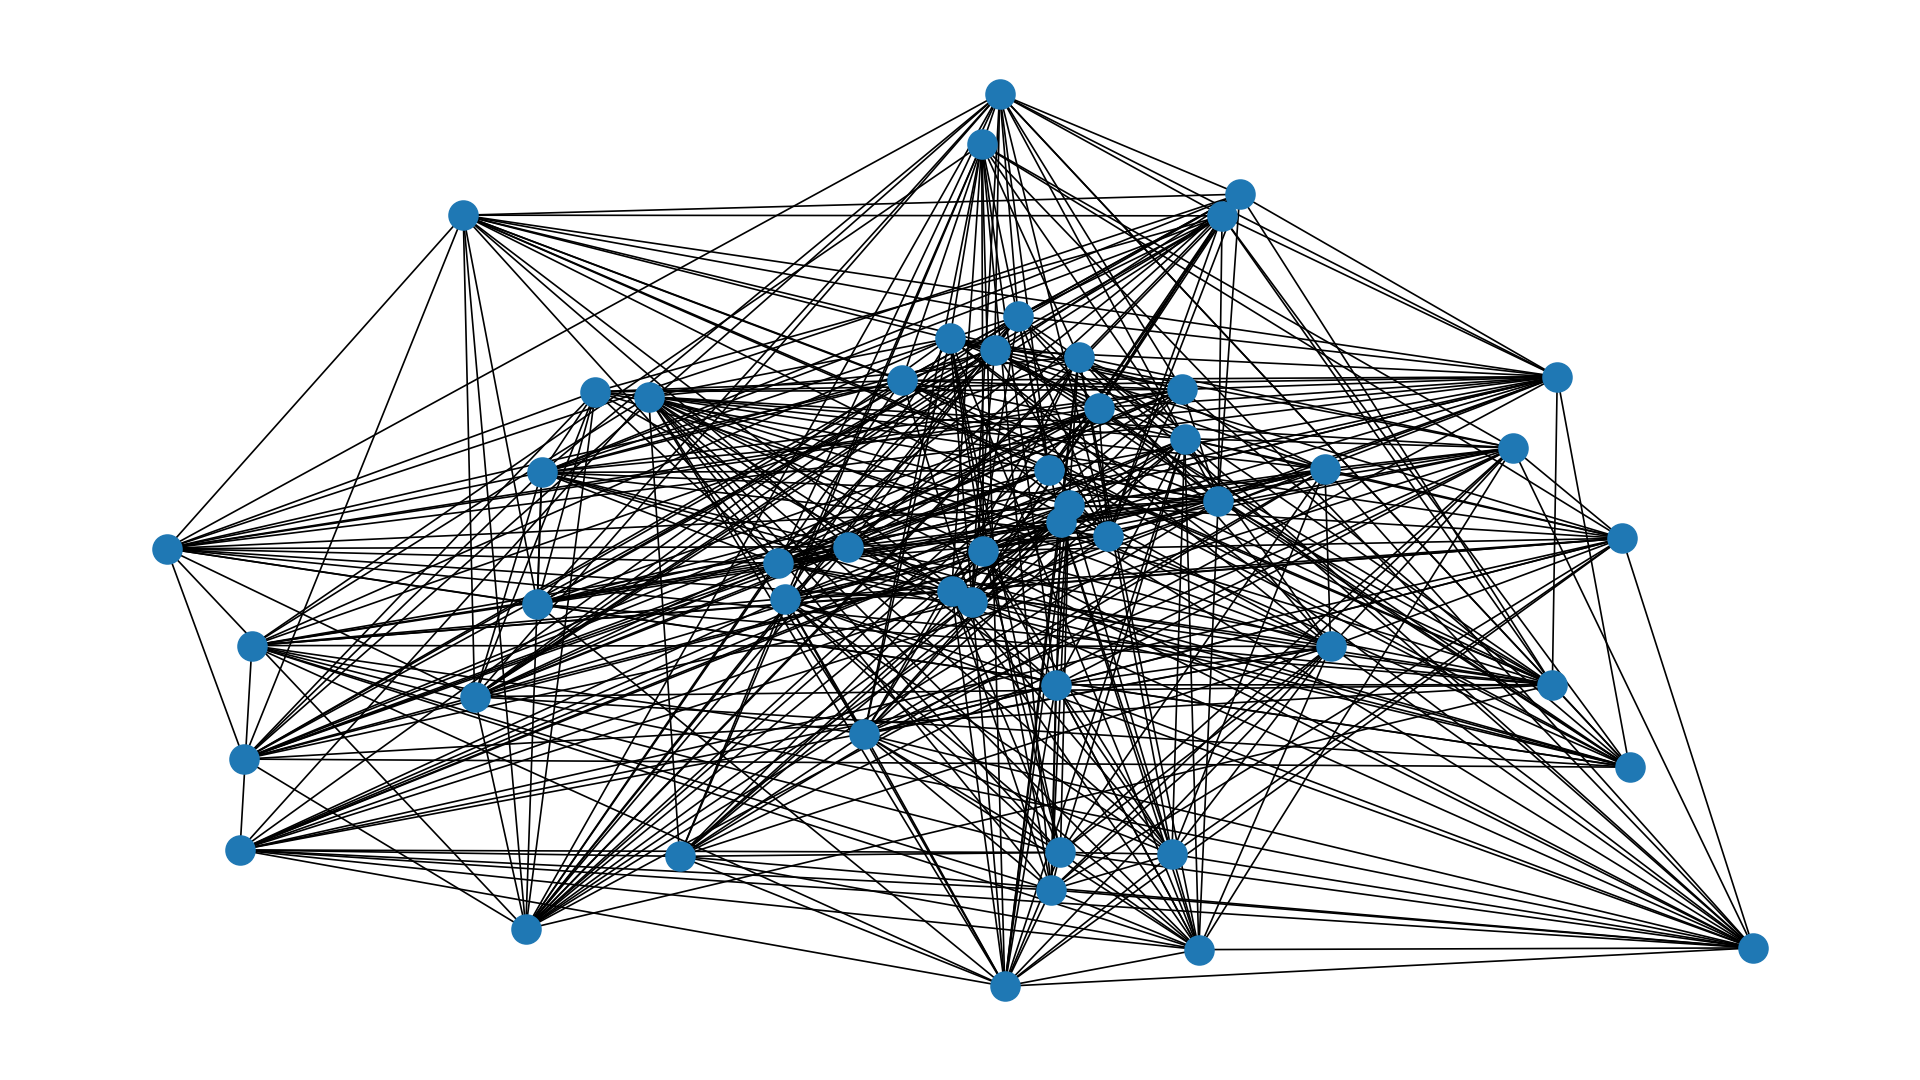
\includegraphics[width=0.9\textwidth]{anim-0}
\end{frame}
\begin{frame}{Graph Drawing Problem}
\centering
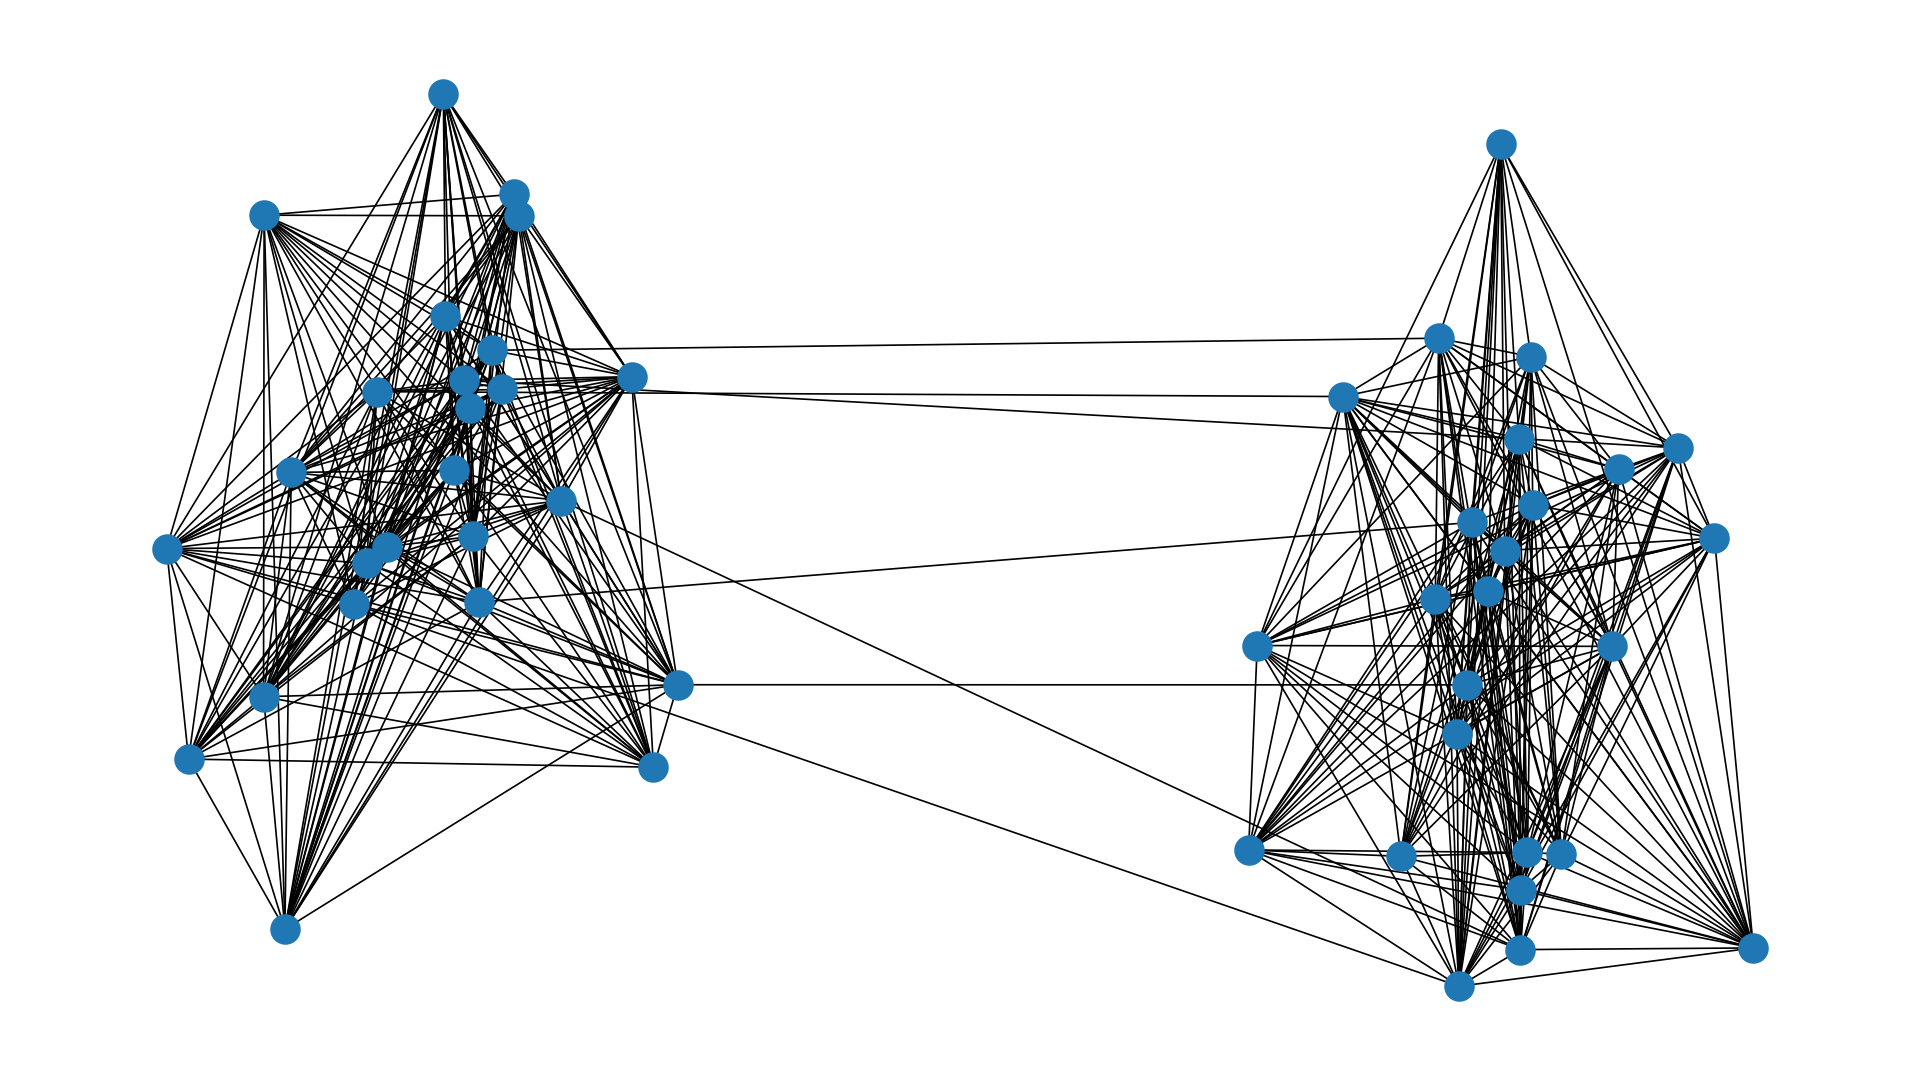
\includegraphics[width=0.9\textwidth]{anim-1}
\end{frame}
%------------------------------------------------

\section{Spectral Graph Theory}
\begin{frame}{Algebraic Connectivity}
\large
\[\lambda_2 = 0 \iff G \text{ is disconnected}\]
\[\hspace{3.1em}\pause\lambda_2 \alert{\approx} 0 \iff G \text{ is \emph{\alert{nearly}} disconnected\alert{?}}\]
% todo: mention algebraic connectivity
\end{frame}

\begin{frame}{Cheeger Constant}
\vspace{-3em}
\centering
\Large
\[h = \min_{S \subseteq V} \max \{\phi(S), \phi(S^c)\}\]
\footnotesize
\[\text{ where } \phi(S) = \frac{\{\text{\# edges leaving } S\}}{\{\text{\# vertices in } S\}}\]
\normalsize
\vspace{1.5em} \\ $h$ tells us how `hard' the Graph is to bisect. 
% todo: give defn but don't read
% todo: mention NP-Hard
\end{frame}

\begin{frame}{First-order Cheeger inequality ($\mathcal{L}$)}
\pause
\vspace{-1em}
\Large
\[
\frac{\lambda_2}{2} \le h \le \sqrt{2\lambda_2}
\]
\centering
\footnotesize Continuous case: \textbf{[Cheeger'70]}. \\ Discrete case: \textbf{[Alon, Milman'85]}.
\vspace{2em}
\normalsize
\pause
\[
\lambda_2 \approx 0 \iff h \approx 0 \iff G \text{ is `nearly disconnected'}
\]
\end{frame}

% todo: graph clustering problem
% todo: mention min-cut NP hard
\section{Higher-order Cheeger Inequalities}
\begin{frame}{Higher-order Cheeger Inequalities}
\centering
Does this generalize for $k > 2$?
\pause
\alert{Yes!}
\[
\frac{\lambda_k}{2} \le h_k \le O(k^2)\sqrt{\lambda_k}
\]
% todo: mention good clusering <=> small eigenvalue
\footnotesize
\textbf{[Lee, Oveis Gharan, Trevisan'14]}
\end{frame}

\begin{frame}{$k$-clustering Problem}
% todo: talk about 'if we have k clusters how do we identify'
% todo: mention the proof of this is algorithmic and leads us to solutions for the k-clustering problem
% todo: mention that good clustering <-> low h_k, hence if we can construct clustering from F we can relate h_k and eigenvalues
% todo: mention that this provides theoretical justification for existing practice
\centering
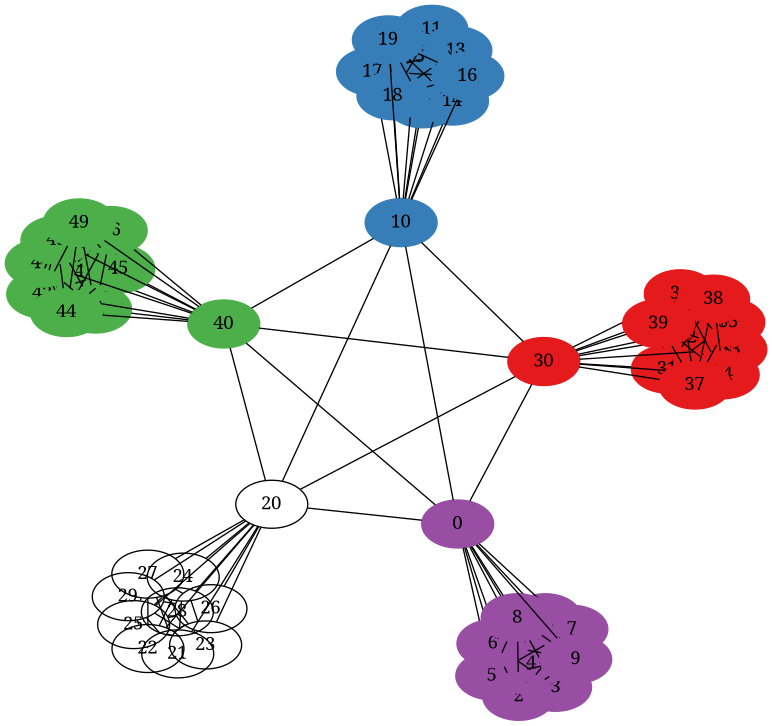
\includegraphics[width=0.5\textwidth]{algo-example}
\end{frame}

\begin{frame}{Proof Overview ($k = 3$)}
\pause
% todo: argue that neighbouring vertices get mapped to close points in R^2 in this embedding
Consider \emph{spectral embedding} $F: V \to \mathbb{R}^2$ given by $F(v) = (f_2(v), f_3(v))$.
\pause
\centering
% todo: mention if we only look along the x axis then the distribution is quite uniform, but if we look along f3 then the structure is revealed
% 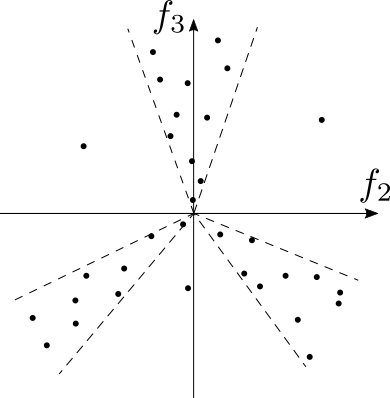
\includegraphics[width=0.4\textwidth]{reproduced-f2-f3}
\def\svgwidth{0.4\columnwidth}
\input{drawing.pdf_tex}
\end{frame}

\begin{frame}{Proof Overview}
\vspace{-2em}
\small
\[\text{\alert{Goal:} Split graph into $k$ clusters to form upper bound on $h_k$}\]
\[\text{Spectral embedding: } F(v) = (f_2(v), f_3(v), \dots, f_k(v))\]
\large
\begin{enumerate}
\item Regions of diameter $\Delta$ contain less than $\frac{1}{k(1-\Delta^2)}$ fraction of vertices
% todo: mention 'regions of given diameter don't contain too many vertices'
% todo: mention that this happens for all orthonormal F
% todo: 'isotropy' / no skew
\normalsize
\[\sum_{v \in V} \langle \hat{x}, F(v) \rangle^2 = 1\]
\large
\pause
\item Apply random partitioning \small\textbf{[Gupta, Krauthgamer, Lee. '03]} \large to achieve well-separated regions
% todo: mention 'to achieve well separated regions of constant diameter covering most of the vertices in the graph'
\large
\pause
\item Form the clustering from vertices within each region
\end{enumerate}
% todo: then use properties of F to make connection to eigenvalues
\end{frame}

\begin{frame}{Applications of Spectral Clustering}
\centering
% todo: mention given image, construct 'similarity matrix'
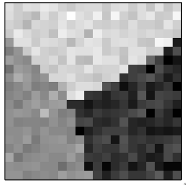
\includegraphics[width=0.20\textwidth]{shi-malik-1} \\
\centering
\vspace{1em}
\pause
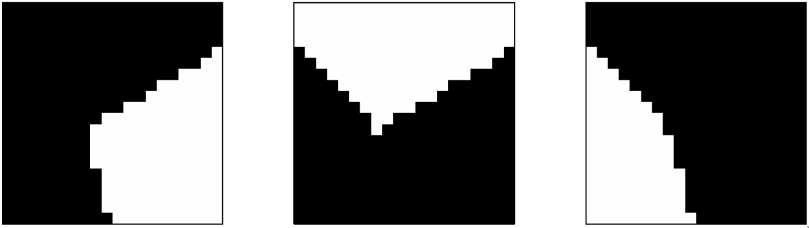
\includegraphics[width=0.6\textwidth]{shi-malik-2} \\
\footnotesize \textbf{[Shi, Malik'00]}
\end{frame}

\begin{frame}
\Huge{\centerline{\textbf{Thank you for listening.}}}
    \footnotesize{
        \begin{thebibliography}{99}
            \centering
            \vspace{3em}
            \bibitem[Chung, 1997]{p1} Fan Chung (1997)
            \newblock Spectral Graph Theory
            \bibitem[Lee, Oveis Gharan, Trevisan'14]{p1} James Lee, Shayan Oveis Gharan, Luca Trevisan (2014)
            \newblock  Multi-way spectral partitioning and higher-order Cheeger inequalities
            \newblock \emph{Journal of the ACM} 
        \end{thebibliography}
    }
\end{frame}
%----------------------------------------------------------------------------------------
\end{document}
